%!TEX root = ../../paper.tex

\Cref{fig:experiment:singlesphere:sets} shows a scatter plot representation of the data sets defined in \cref{tab:experiment:singlesphere:sets}. The slices of the eigenellipsoids of the Gaussian components in \cref{fig:experiment:singlesphere:projection} emphasize the differences between the data sets. It should be noted that the lengths of the major axes of data set \baakmanOne through \baakmanFive are the squared length of the major axis of set \ferdosiOne.

\begin{figure}[b!]
	\centering
	%!TEX root = ../../paper.tex

%Ferdosi Sets 1
\begin{subfigure}{0.23\columnwidth}
	\centering
	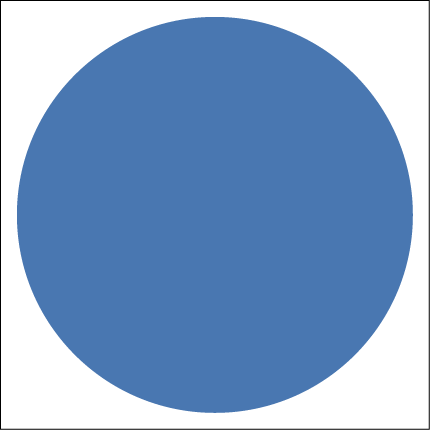
\includegraphics[width=\textwidth]{experiment/img/singlesphereimpression_ferdosi1.png}
	\caption{Set \ferdosiOne}
	\label{fig:experiment:singlesphere:projection:ferdosi1}
\end{subfigure}
% Baakman 1	
\begin{subfigure}{0.23\columnwidth}
	\centering
	
\includegraphics[width=\textwidth]{experiment/img/singlesphereimpression_baakman1.png}
	\caption{Set \baakmanOne}
	\label{fig:experiment:singlesphere:projection:baakman1}
\end{subfigure}
% Baakman 4
\begin{subfigure}{0.23\columnwidth}
	\centering
	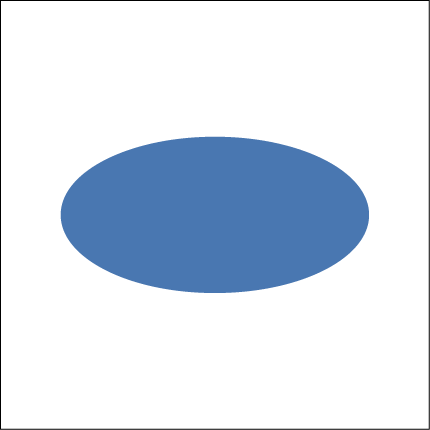
\includegraphics[width=\textwidth]{experiment/img/singlesphereimpression_baakman4.png}
	\caption{Set \baakmanFour}
	\label{fig:experiment:singlesphere:projection:baakman4}
\end{subfigure}	
% Baakman 5
\begin{subfigure}{0.23\columnwidth}
	\centering
	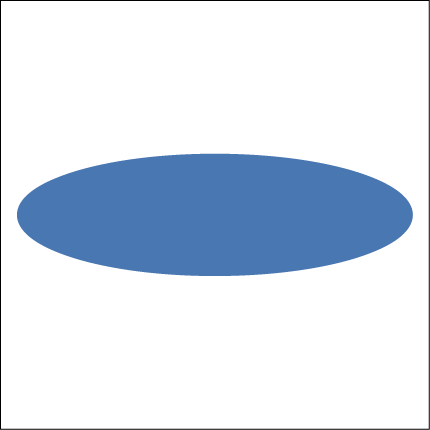
\includegraphics[width=\textwidth]{experiment/img/singlesphereimpression_baakman5.png}
	\caption{Set \baakmanFive}
	\label{fig:experiment:singlesphere:projection:baakman5}
\end{subfigure}	
	\caption{Slice of the $y,z$-plane of the eigenellipsoid of the Gaussian component of data set%
		\subref{fig:experiment:singlesphere:projection:ferdosi1} \ferdosiOne, %
		\subref{fig:experiment:singlesphere:projection:baakman1} \baakmanOne, %
		\subref{fig:experiment:singlesphere:projection:baakman4} \baakmanFour, and %
		\subref{fig:experiment:singlesphere:projection:baakman5} \baakmanFive %
		 at $x = 50$.}
	\label{fig:experiment:singlesphere:projection}
\end{figure}

% General
The Gaussian components of these data sets progress from a sphere, \ie data set \ferdosiOne, to an increasingly elongated ellipsoid. This makes it possible to investigate the influence of how strongly elongated the distribution is, on the density estimate.
	% Ferdosi One
	The first data set is a spherical Gaussian distribution centered in a uniform random background.
	% Baakman One
	The covariance matrix of the Gaussian component in \baakmanOne is created from the covariance matrix used in \ferdosiOne by squaring one of its eigenvalues, and taking the square root of the other two eigenvalues, without changing the eigenvectors. The resulting covariance matrix defines an eigenellipse with the same volume as the one defined by \ferdosiOne.
	% Baakman Four
	The Gaussian component of data set \baakmanFour changes the shape of the eigenellipsoid of the Gaussian component in set \ferdosiOne by lengthening one of the minor axes, and shortening the minor axis.
	% Baakman Five
	In data set \baakmanFive the Gaussian component is spread out more along the $y$-axis and less along the $z$-axis, than the Gaussian component in data set \baakmanFour.

% Hypothesis
	% Ferdosi 1
	We expect the Modified Breiman Estimator and its shape-adaptive cousin to perform comparably on data set \ferdosiOne, since the symmetric shape of the Gaussian distribution means no advantage should be gained by using a shape-adaptive kernel and nor should it do much steering.
	% Baakman 1, 4, 5
	As the Gaussian distribution is more and more elongated, the advantages of using \sambe should become more pronounced.